\documentclass{beamer}

\usetheme{Pittsburgh}
\usecolortheme{beaver}

\usepackage{dot2texi}
\usepackage{tikz}
\usetikzlibrary{shapes,arrows}
\usepackage{bookmark}
\usepackage{graphicx}
\usepackage{todonotes}

\mode<handout>{%
  \usepackage{pgfpages}
  \pgfpagesuselayout{resize to}[a4paper]
}

\title{Building a Web Search}
\author{Ross Fenning}
\institute{
  Senior Software Engineer
  \\Content Discovery
  \\Future Media
  \\BBC
}
\date{17 June, 2014}

\begin{document}

\begin{frame}[plain]
  \titlepage
\end{frame}

% Background
\begin{frame}
  \frametitle{About Me}
  \begin{itemize}
    \pause \item Senior Software Engineer
    \pause \item BBC Future Media
    \pause \item Content Discovery: Search
    \pause \item BBC Academy and University of Bradford, UK
    \pause \item Bournemouth University, UK and Lancaster University
    \pause \item School of Design Engineering \& Computing at Bournemouth University
  \end{itemize}
\end{frame}

\begin{frame}
  \frametitle{What is BBC Search?}
  \framesubtitle{i.e. What do I work on?}
  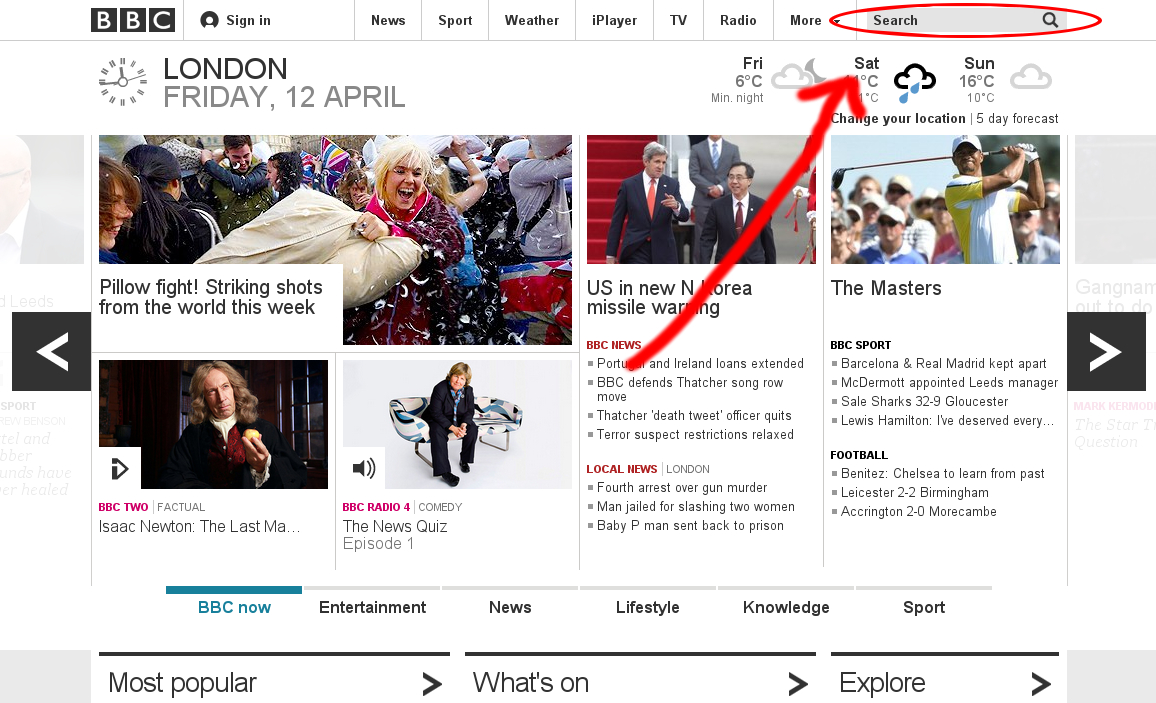
\includegraphics[width=\linewidth]{homepage.png}
\end{frame}

\begin{frame}
  \frametitle{Why BBC Search?}
  \framesubtitle{Isn't Google good enough?}
  \begin{itemize}
    \pause \item We can search the BBC via Google
    \pause \item What can the BBC offer that Google cannot?
    \pause \item Domain knowledge about our own content
    \pause \item More ``real time'' updates of content
  \end{itemize}
\end{frame}

% Design Goals
\begin{frame}
  \frametitle{Design Goals}
  \begin{itemize}
    \pause \item Existing search application serves a wide variety of use cases
    \pause \item Start high-level thinking and design of a new search application
    \pause \item Take a ``fresh'' approach as if we are replacing the whole system
    \pause \item A new design can (hopefully) inform iterative improvements on a current system
    \pause \item Can SSM give us contextualisation that applies both to a new application and to existing systems?
    \pause \item The Search application should integrate where possible with other existing systems
    \pause \item Can SSM helps us consider the holistic search system that emerges after this integration?
  \end{itemize}
\end{frame}

% Contextualisation of the problems space through SSM
\begin{frame}
  \frametitle{Problem Contextualisation through SSM}
  \begin{itemize}
    \pause \item Claim: ``Hard systems'' (e.g. UML) take an ontological view:
    \begin{itemize}
      \pause \item What components are there?
      \pause \item Who are the actors?
      \pause \item What are the interactions between actors and components?
      \pause \item What are the computations or workflows steps/stages?
    \end{itemize}
    \pause \item Claim: SSM takes an epistemological view:
    \begin{itemize}
      \pause \item How does the holistic search system transform user needs to content and information?
      \pause \item How can the purposeful activity be monitored?
      \pause \item How is the activity observed by different observers?
      \pause \item How can different observers inform the activity?
    \end{itemize}
    \pause \item Interactive Management (Dogan and Henshaw, 2010) can capture requirements and transition to formal models
  \end{itemize}
\end{frame}

\begin{frame}
  \frametitle{Problem Contextualisation through SSM}
  \framesubtitle{Rich Picture}
  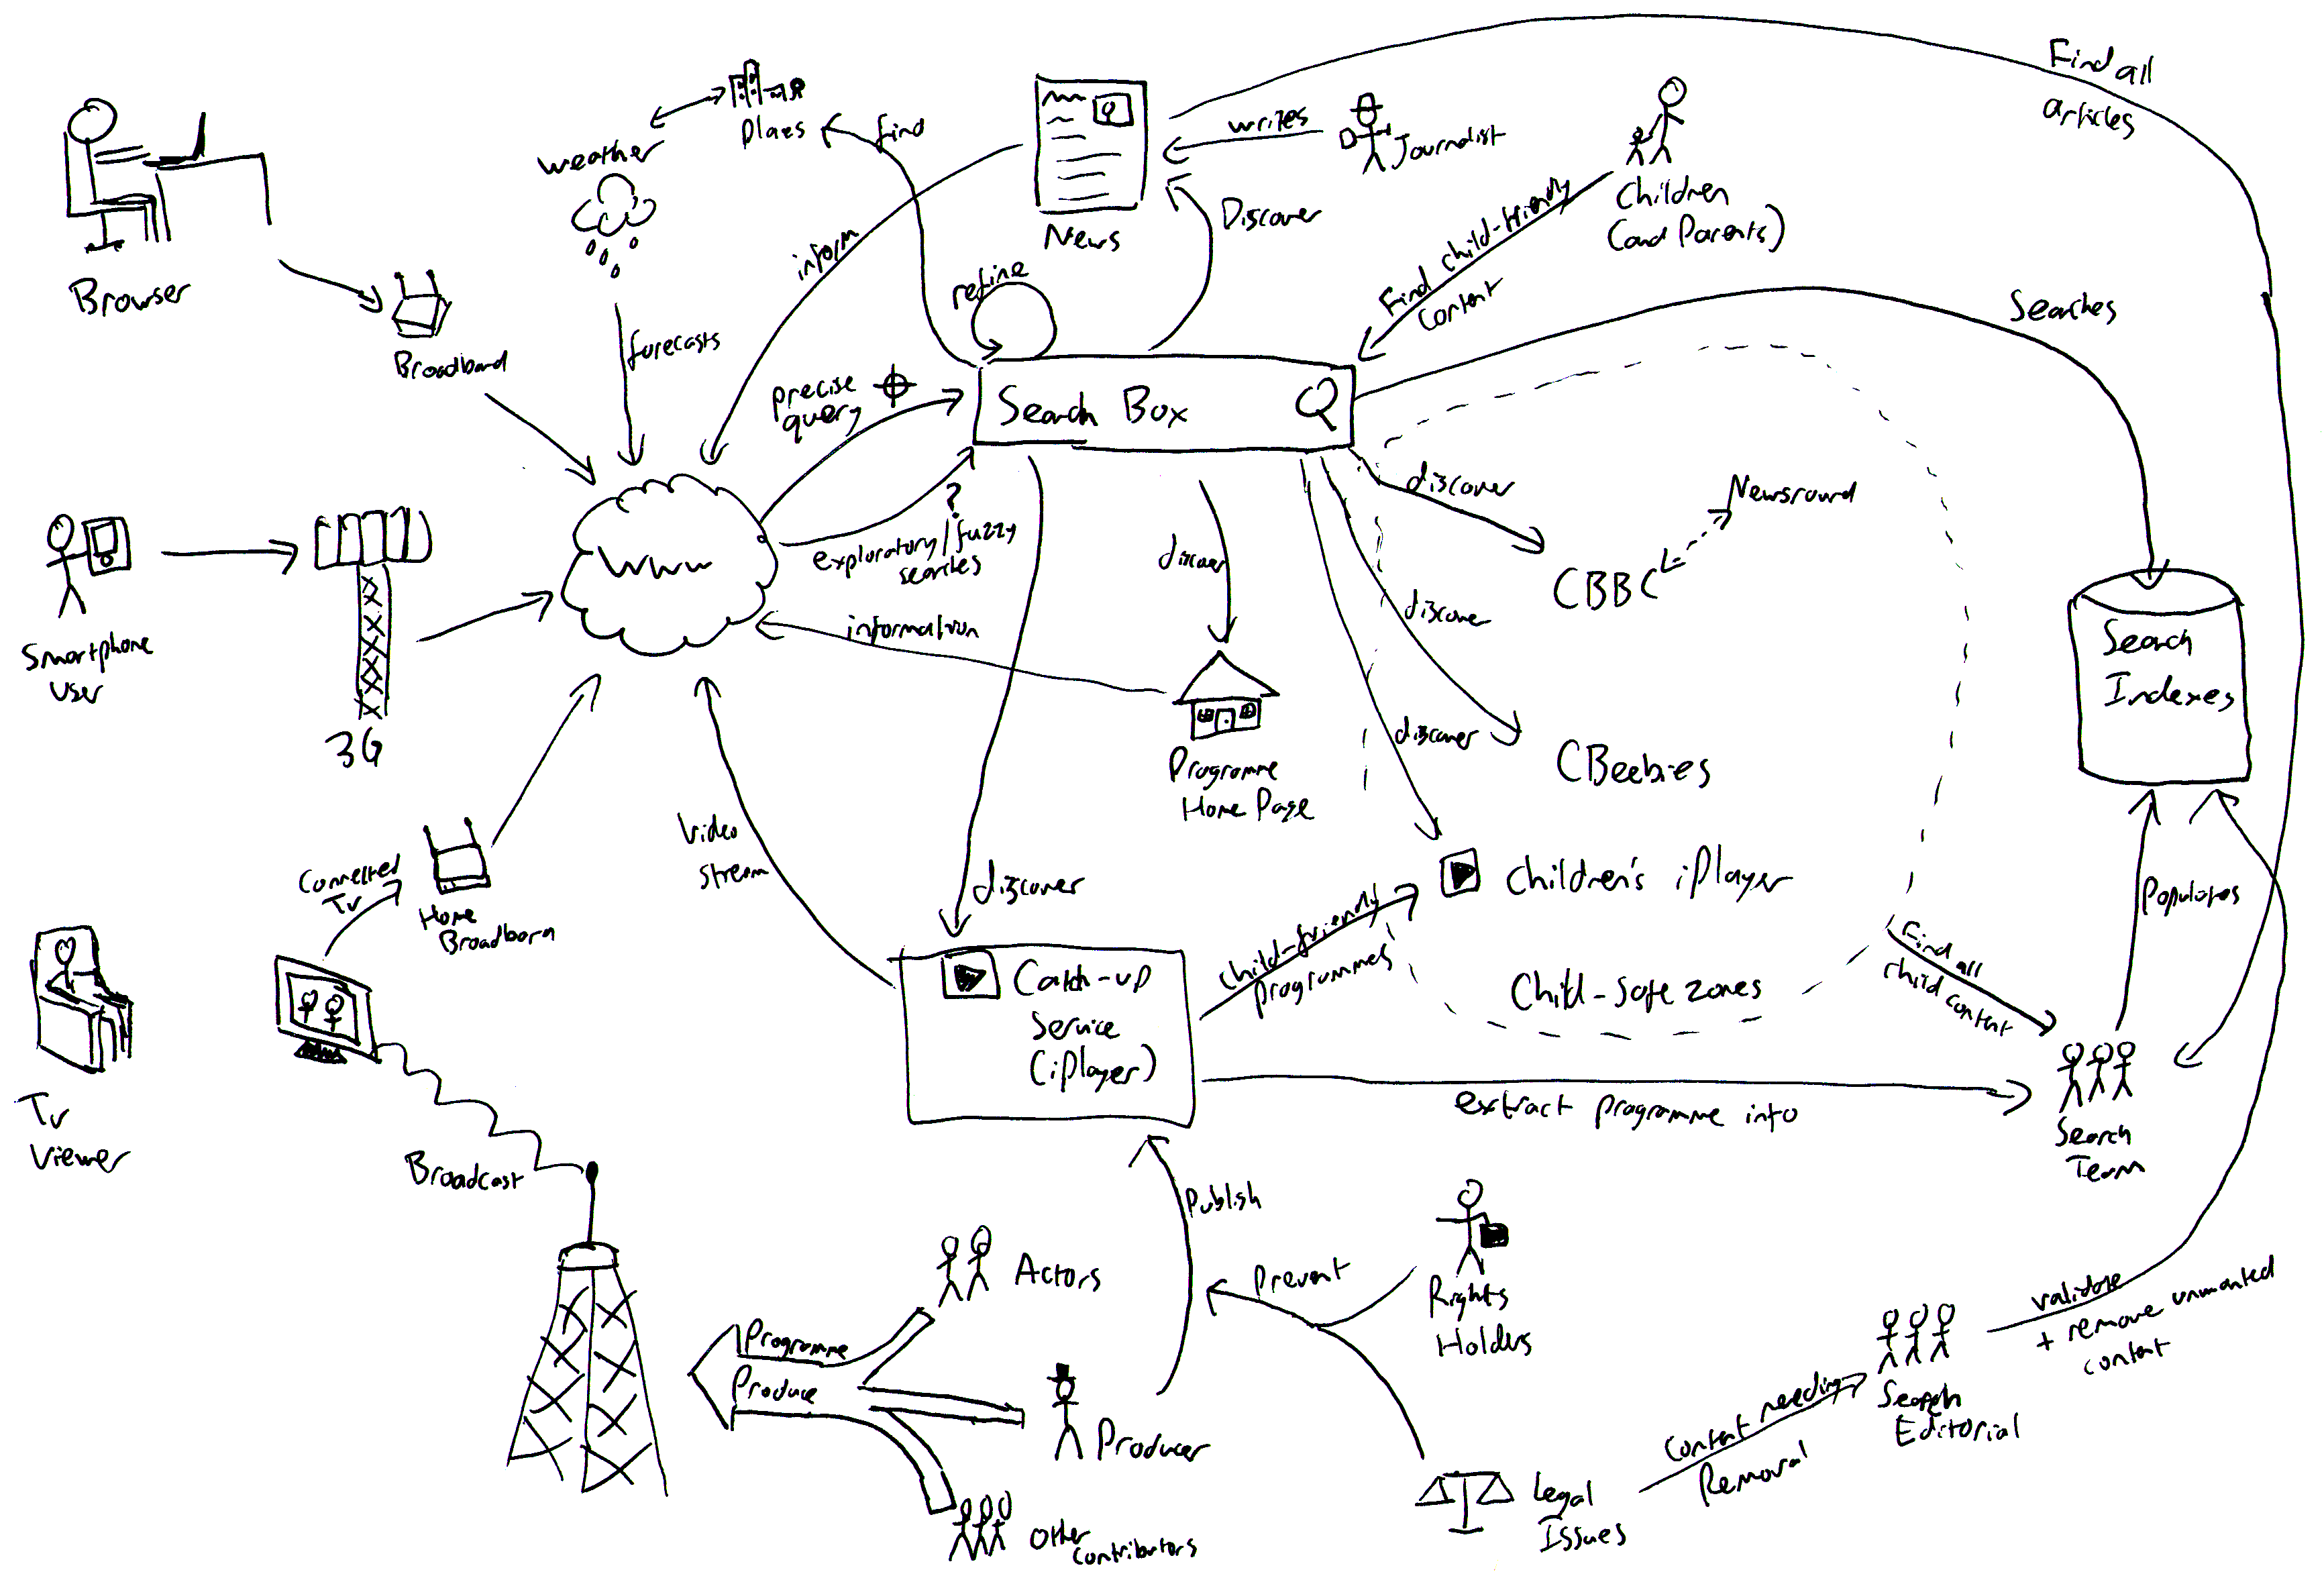
\includegraphics[width=\linewidth]{rich-picture.png}
\end{frame}

% Extracting use cases
\begin{frame}
  \frametitle{Use Case Extraction}
  \framesubtitle{Identifying users}
  \begin{itemize}
    \pause \item Identifier all users of the system in the rich picture
    \pause \item Separate \emph{direct} users from \emph{meta-level} users
    \pause \item Direct use cases should emerge from the rich picture
    \pause \item This separation is still \emph{subjective} and use cases may change as the rich picture changes
  \end{itemize}
\end{frame}

% Designing behaviour for indirect users
\begin{frame}
  \frametitle{Use Case Extraction}
  \framesubtitle{Meta-level Users}
  \begin{itemize}
    \pause \item Meta-level users do not transition to the use case models directly
    \pause \item \emph{Systems Thinking} tells us to consider how meta-level users are affected by emergent properties of the holistic system
  \end{itemize}
\end{frame}

% Designing behaviour for direct users
\begin{frame}
  \frametitle{Use Case Extraction}
  \framesubtitle{Direct Users}
  \begin{itemize}
    \pause \item Direct users transition directly to actors into a UML use case diagram
    \pause \item Use cases should derive from and be justifiable by the rich picture
    \pause \item Direct users divide up into \emph{content production} and \emph{audience}
    \pause \item Examples of each:
    \begin{itemize}
      \pause \item Producers of TV programmes metadata
      \pause \item Users of the search web application
    \end{itemize}
  \end{itemize}
\end{frame}

% Domain modelling for search -- model business rules as per benefits shown in background, but also keep it generic
% Discussion and Analysis -- Use cases - More SSM needed?
% Discussion and Analysis -- Domain Model -- Polymorphism
% Discussion and Analysis -- Domain Model -- Duck Typing
% Discussion -- More SSM: 3 Es?
% Shortcomings -- Performance? NFRs?
% Shortcomings -- Agile?
% Validation?

\end{document}
